\chapter{Lists}\label{ch:lists}

\tikzset{
  lcell/.style={draw,minimum width=7mm,minimum height=6mm,inner sep=1pt},
  lptr/.style={-{Stealth}},
  rarr/.style={-{Stealth},thick},
  rcall/.style={draw,rounded corners,fill=blue!6,font=\ttfamily\small,minimum height=6mm},
  rval/.style={draw,rounded corners,fill=green!8,font=\ttfamily\small,minimum height=6mm,minimum width=8mm}
}

Structures hold a \emph{fixed} number of values. To represent an arbitrary
number of values --- a class list, the words in a sentence, a sequence of
measurements --- we need a type whose values can be any size. The list is
the fundamental such type in Racket.

\section{Constructing lists}

A list is either empty, or a first element followed by the rest of the list.
\begin{itemize}
  \item \code{empty} (also written \code{'()}) is the empty list.
  \item \code{(cons v lst)} produces a new list whose first element is \code{v} and whose rest is the list \code{lst}.
\end{itemize}

\begin{lstlisting}[style=racket]
empty                                  ; the empty list
(cons 'a empty)                        ; one element
(cons 'a (cons 'b (cons 'c empty)))    ; three elements: a, b, c
\end{lstlisting}

\begin{center}
\begin{tikzpicture}[node distance=0pt,
  cell/.style={draw, minimum width=7mm, minimum height=6mm}]
  \node[cell] (a1) {\texttt{'a}}; \node[cell, right=of a1] (a2) {};
  \node[cell, right=12mm of a2] (b1) {\texttt{'b}}; \node[cell, right=of b1] (b2) {};
  \node[cell, right=12mm of b2] (c1) {\texttt{'c}}; \node[cell, right=of c1] (c2) {};
  \node[right=12mm of c2] (e) {\texttt{empty}};
  \draw[-{Stealth}] (a2.center) -- (b1.west);
  \draw[-{Stealth}] (b2.center) -- (c1.west);
  \draw[-{Stealth}] (c2.center) -- (e.west);
\end{tikzpicture}
\end{center}

\section{Deconstructing lists}
\begin{itemize}
  \item \code{(first lst)} --- the first element; error on \code{empty}.
  \item \code{(rest lst)} --- the list without its first element; error on \code{empty}.
  \item \code{(empty? v)} --- true iff \code{v} is the empty list.
  \item \code{(cons? v)} --- true iff \code{v} is a non-empty list.
\end{itemize}

\begin{important}[List substitution rules]
\begin{itemize}
  \item \code{(first (cons a b))} $\Rightarrow$ \code{a}
  \item \code{(rest (cons a b))} $\Rightarrow$ \code{b}
  \item \code{(empty? empty)} $\Rightarrow$ \code{true}; \code{(empty? v)} $\Rightarrow$ \code{false} for any other value
  \item \code{(cons? (cons a b))} $\Rightarrow$ \code{true}; \code{(cons? v)} $\Rightarrow$ \code{false} otherwise
\end{itemize}
A value \code{(cons v1 (cons v2 empty))} is fully evaluated: \code{cons} is a constructor.
\end{important}

\section{Data definition for lists}

The set of lists is defined \textbf{recursively} (self-referentially):

\begin{lstlisting}[style=racket]
;; A (listof Num) is one of:
;; * empty
;; * (cons Num (listof Num))
\end{lstlisting}

Drawn as nested boxes, each non-empty list holds a first element and,
inside it, a smaller list --- until the innermost box is \code{empty}:

\begin{center}
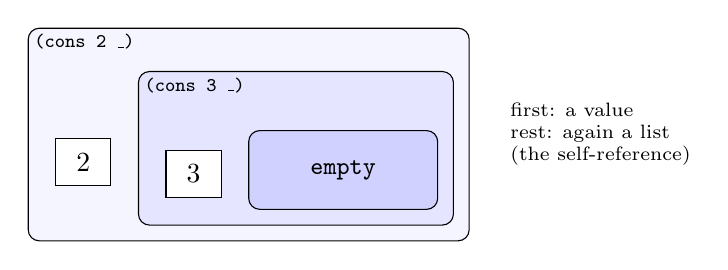
\begin{tikzpicture}[lab/.style={font=\scriptsize\ttfamily,anchor=north west,inner sep=2pt}]
  \draw[rounded corners,fill=blue!4] (0,0) rectangle (5.6,2.7);
  \node[lab] at (0,2.7) {(cons 2 \_)};
  \node[lcell,fill=white] at (0.7,1.0) {2};
  \draw[rounded corners,fill=blue!10] (1.4,0.2) rectangle (5.4,2.15);
  \node[lab] at (1.4,2.15) {(cons 3 \_)};
  \node[lcell,fill=white] at (2.1,0.85) {3};
  \draw[rounded corners,fill=blue!18] (2.8,0.4) rectangle (5.2,1.4);
  \node[font=\ttfamily\small] at (4.0,0.9) {empty};
  \node[font=\scriptsize,align=left,anchor=west] at (6.0,1.35) {first: a value\\rest: again a list\\(the self-reference)};
\end{tikzpicture}
\end{center}

The definition is not circular because the base case \code{empty} is not
self-referential, and every self-reference refers to a smaller list. We use
\code{(listof X)} for any element type \code{X}, and sometimes
\code{(ne-listof X)} for non-empty lists:

\begin{lstlisting}[style=racket]
;; A (ne-listof X) is one of:
;; * (cons X empty)
;; * (cons X (ne-listof X))
\end{lstlisting}

\section{The list template}

The template follows the data definition: one \code{cond} clause per case,
selectors in the \code{cons} case, and --- because the rest is itself a list
--- a \textbf{recursive call} on the rest.

\begin{lstlisting}[style=racket]
;; listof-X-template: (listof X) -> Any
(define (listof-X-template lst)
  (cond [(empty? lst) ...]
        [(cons? lst) (... (first lst) ...
                          (listof-X-template (rest lst)) ...)]))
\end{lstlisting}

\begin{important}[Key idea]
Assume the recursive call already produces the correct answer for
\code{(rest lst)}. Your job is only to say how to combine \code{(first lst)}
with that answer. This is the programming analogue of the induction step in
a proof by induction.
\end{important}

\section{First recursive functions}

\begin{example}[Counting elements]
\begin{lstlisting}[style=racket]
;; (count-items lst) produces the number of elements in lst.
;; Examples:
(check-expect (count-items empty) 0)
(check-expect (count-items (cons 'a (cons 'b empty))) 2)

;; count-items: (listof Any) -> Nat
(define (count-items lst)
  (cond [(empty? lst) 0]
        [else (+ 1 (count-items (rest lst)))]))
\end{lstlisting}
(This is the built-in \code{length}.)
\end{example}

\begin{example}[Sum]
\begin{lstlisting}[style=racket]
;; (sum lst) produces the sum of the numbers in lst.
;; Examples:
(check-expect (sum empty) 0)
(check-expect (sum (cons 2 (cons 3 empty))) 5)

;; sum: (listof Num) -> Num
(define (sum lst)
  (cond [(empty? lst) 0]
        [else (+ (first lst) (sum (rest lst)))]))
\end{lstlisting}
\end{example}

\paragraph{Condensed trace.} Full traces of recursive functions are long; a
\emph{condensed trace} shows only the key steps:
\begin{lstlisting}[style=racket]
(sum (cons 2 (cons 3 empty)))
=> (+ 2 (sum (cons 3 empty)))
=> (+ 2 (+ 3 (sum empty)))
=> (+ 2 (+ 3 0))
=> (+ 2 3)
=> 5
\end{lstlisting}
The same computation as a picture: the calls go down the list one
\code{rest} at a time, and the answers come back up, each level adding its
own first element.

\begin{center}
\begin{tikzpicture}
  \node[rcall] (c1) at (0,0) {(sum (list 2 3))};
  \node[rcall] (c2) at (0,-1.2) {(sum (list 3))};
  \node[rcall] (c3) at (0,-2.4) {(sum empty)};
  \node[rval] (r3) at (5,-2.4) {0};
  \node[rval] (r2) at (5,-1.2) {3};
  \node[rval] (r1) at (5,0) {5};
  \draw[rarr] (c1) -- node[left,font=\scriptsize]{rest} (c2);
  \draw[rarr] (c2) -- node[left,font=\scriptsize]{rest} (c3);
  \draw[rarr] (c3) -- node[above,font=\scriptsize]{base case} (r3);
  \draw[rarr,green!40!black] (r3) -- node[right,font=\scriptsize\ttfamily]{(+ 3 0)} (r2);
  \draw[rarr,green!40!black] (r2) -- node[right,font=\scriptsize\ttfamily]{(+ 2 3)} (r1);
  \draw[densely dotted] (c1) -- (r1);
  \draw[densely dotted] (c2) -- (r2);
\end{tikzpicture}
\end{center}

For comparison, the first few full steps are:
\begin{lstlisting}[style=racket]
(sum (cons 2 (cons 3 empty)))
=> (cond [(empty? (cons 2 (cons 3 empty))) 0]
         [else (+ (first (cons 2 (cons 3 empty)))
                  (sum (rest (cons 2 (cons 3 empty)))))])
=> (cond [false 0]
         [else (+ (first (cons 2 (cons 3 empty)))
                  (sum (rest (cons 2 (cons 3 empty)))))])
=> (cond [else (+ (first (cons 2 (cons 3 empty)))
                  (sum (rest (cons 2 (cons 3 empty)))))])
=> (+ (first (cons 2 (cons 3 empty))) (sum (rest (cons 2 (cons 3 empty)))))
=> (+ 2 (sum (rest (cons 2 (cons 3 empty)))))
=> (+ 2 (sum (cons 3 empty)))
=> ...
\end{lstlisting}

\section{List abbreviations}
In \emph{Beginning Student with List Abbreviations}:
\begin{itemize}
  \item \code{(list 1 2 3)} abbreviates \code{(cons 1 (cons 2 (cons 3 empty)))}.
  \item \code{'(a b c)} abbreviates \code{(list 'a 'b 'c)}; quoting distributes over the elements.
  \item \code{second}, \code{third}, \ldots, \code{eighth} select later elements.
\end{itemize}
\code{(list 1 2)} and \code{(cons 1 2)} are different: the latter is not a list
at all in the teaching languages (it is an error, since the second argument
must be a list). \code{(cons (list 1 2) (list 3))} is the two-element list
\code{(list (list 1 2) 3)}.

In box-and-pointer form, the first element of the outer list is itself a
pointer to the inner list:

\begin{center}
\begin{tikzpicture}
  \node[lcell] (a1) at (0,0) {}; \node[lcell] (a2) at (0.7,0) {};
  \node[lcell] (b1) at (2.1,0) {3}; \node[lcell] (b2) at (2.8,0) {};
  \node[font=\ttfamily\small] (e1) at (4.3,0) {empty};
  \node[lcell] (c1) at (0,-1.4) {1}; \node[lcell] (c2) at (0.7,-1.4) {};
  \node[lcell] (d1) at (2.1,-1.4) {2}; \node[lcell] (d2) at (2.8,-1.4) {};
  \node[font=\ttfamily\small] (e2) at (4.3,-1.4) {empty};
  \fill (a1.center) circle (1.2pt);
  \draw[lptr] (a1.center) -- (c1.north);
  \draw[lptr] (a2.center) -- (b1.west);
  \draw[lptr] (b2.center) -- (e1.west);
  \draw[lptr] (c2.center) -- (d1.west);
  \draw[lptr] (d2.center) -- (e2.west);
  \node[font=\scriptsize,anchor=east] at (-0.5,0) {outer list};
  \node[font=\scriptsize,anchor=east] at (-0.5,-1.4) {\code{(list 1 2)}};
\end{tikzpicture}
\end{center}

\section{Lists of structures and strings}

Lists can hold any values. A list of structures uses both templates together:
\begin{lstlisting}[style=racket]
;; (class-average los) produces the average avg of the students in los.
;; class-average: (listof Student) -> Num
;;   requires: los is non-empty
(define (class-average los)
  (/ (total-avg los) (length los)))

;; (total-avg los) produces the sum of the averages in los.
;; total-avg: (listof Student) -> Num
(define (total-avg los)
  (cond [(empty? los) 0]
        [else (+ (student-avg (first los)) (total-avg (rest los)))]))
\end{lstlisting}

Strings are processed by converting to a list of characters:
\begin{lstlisting}[style=racket]
;; (count-vowels s) produces the number of vowels in s.
;; count-vowels: Str -> Nat
(check-expect (count-vowels "banana") 3)
(define (count-vowels s) (count-vowels/list (string->list s)))

;; count-vowels/list: (listof Char) -> Nat
(define (count-vowels/list loc)
  (cond [(empty? loc) 0]
        [(vowel? (first loc)) (+ 1 (count-vowels/list (rest loc)))]
        [else (count-vowels/list (rest loc))]))

;; vowel?: Char -> Bool
(define (vowel? c) (member? (char-downcase c) '(#\a #\e #\i #\o #\u)))
\end{lstlisting}

\section{Common pitfalls}
\begin{itemize}
  \item Taking \code{first} or \code{rest} of \code{empty}.
  \item Forgetting the base case, or getting its value wrong (the sum of nothing is 0, the product of nothing is 1).
  \item Confusing \code{cons} (add one element at the front) with \code{append} (join two lists).
  \item Making the recursive call on the whole list instead of the rest (infinite recursion).
\end{itemize}

\section{Summary}
\begin{itemize}
  \item A list is \code{empty} or \code{(cons first rest)}; the data definition is recursive.
  \item The list template has an \code{empty} case and a \code{cons} case with a recursive call on the rest.
  \item Trust the recursion: combine the first element with the answer for the rest.
  \item \code{list} and quote are abbreviations for nested \code{cons}.
\end{itemize}
